\section{Literature Review}\label{sec:litreview}
A number of academic and commercial groups have shown interest in the concept of developing a space-based ADS-B receiver network. Globalstar and Iridium have committed to delivering constellations with full global coverage, piggybacking on their satellite phone network. Thales, ESA and GomSpace have each developed their own small-satellite ADS-B receivers.

\subsection{ADS-B Link Augmentation System (ALAS)}
ADS-B Technologies have developed the ALAS as a space-based ADS-B coverage solution. The ALAS will be flown as hosted payloads on the Globalstar's second generation constellation of satellites. The system is expected to provide global coverage with a one-second update rate \cite{ADS-B:Globalstar_webinar}.

The ALAS is intended to operate by relaying ADS-B data (received via the normal L and S band transmissions) to ground based gateways through the C band. These gateways would then relate that data to Air Traffic Management (ATM) systems as necessary. The system would be full duplex and is designed to transparently augment the existing ADS-B ground coverage network. This operation is illustrated in Figure \ref{fig:alas_overview}
\begin{figure}[htbp]
	\centering
	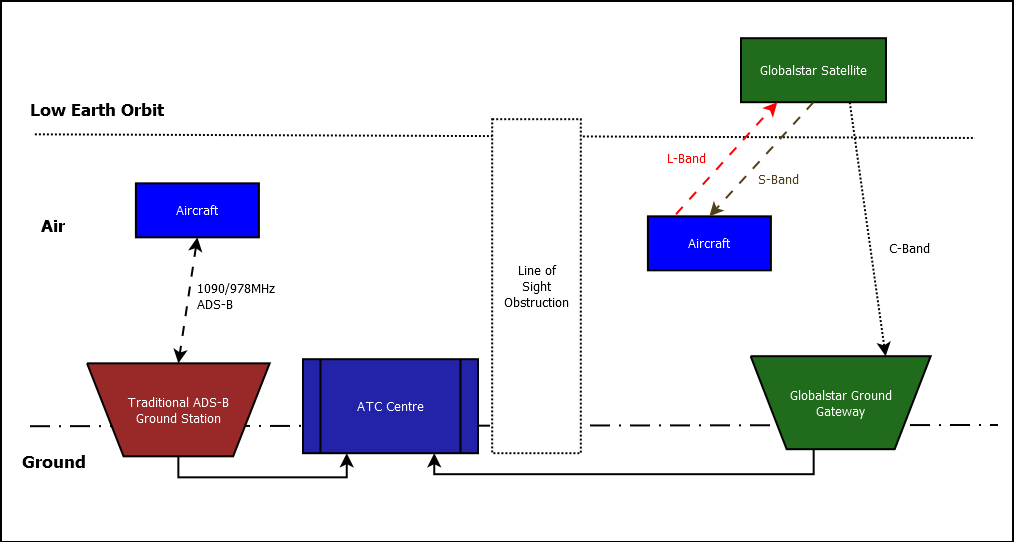
\includegraphics[scale = 0.40]{Pictures/alas_overview_tn.png}
	
	\caption[Overview of the ALAS system]{Overview of the ALAS system, after \cite{ADS-B:Globalstar_webinar}}
	\label{fig:alas_overview}
\end{figure}
This is intended to be an indirect link that requires on-board aircraft to install additional C-band transponders. In this sense it would not be a true `drop in' service. Complete ADS-B coverage using this system would incur significant cost to pilots and aircraft manufacturers.

ADS-B Technologies reported that the second generation Globalstar constellation will provide coverage over most continental areas, with minimal coverage over international waters \cite{ADS-B:Globalstar_webinar}. This is illustrated in Figure \ref{fig:globalstar_adsb}.
\begin{figure}[H]
	\centering
	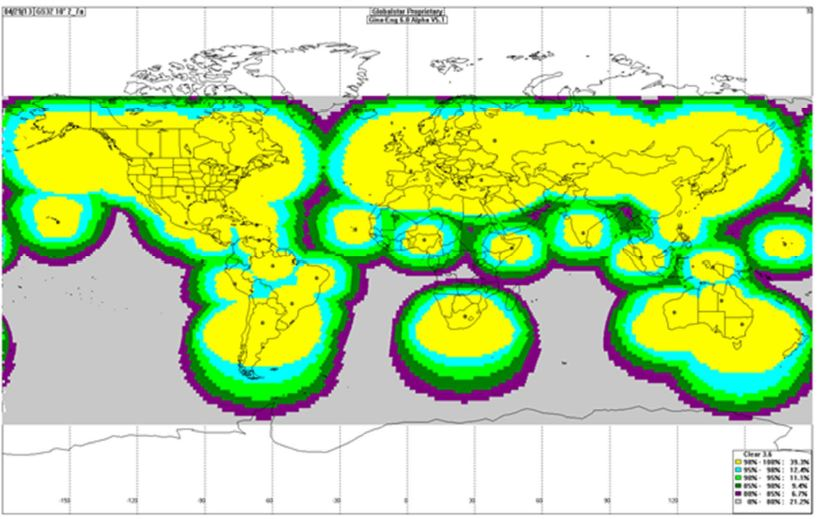
\includegraphics[scale = 0.7]{Pictures/globalstar_asdb.jpg}
	
	\caption[ADS-B Duplex coverage provided by the second generation Globalstar constellation]{ADS-B Duplex coverage provided by the second generation Globalstar constellation, reproduced from \cite{ADS-B:Globalstar_webinar}}
	\label{fig:globalstar_adsb}
\end{figure} 

ALAS would have two major shortcomings -
\begin{enumerate}
	\item The system would require both ANSPs and Aircraft to purchase additional L and S band transceivers to communicate with the space segment. ALAS would not be compatible with standard ADS-B hardware implementation. 
	\item The second Globalstar constellation would have limited coverage due to its orbit configuration and communication infrastructure. The inclination of the Globalstar orbits would not provide ADS-B coverage over the poles, and would rely on a permanent link with ground stations restricts the predicted coverage to continental areas. This is illustrated in Figure \ref{fig:globalstar_adsb}.
\end{enumerate}

ALAS is expected to be operational in late 2014 \cite{ADS-B:Globalstar_webinar}. ADS-B Technologies have not yet released any information about buy-in models for ANSPs.

\subsection{Aireon} \label{sec:aireon}
As of June 2014, Aireon LLC were developing an space-based, ADS-B reliant `global aviation surveillance system' \cite{ADS-B:Aireon_brochure} to be flown on the Iridium NEXT constellation of LEO satellites. The constellation was expected to provide complete global coverage, including over polar regions \cite{ADS-B:Aireon_comparison}.   

This system was presented as flight path solutions for both ANSPs and commercial airlines. Marketing material claimed that intelligent flight path planning will save airlines fuel costs with more optimised routes \cite{ADS-B:Aireon_comparison}. No independent analyses or verifications of these claims were found. The service was expected to be available by 2017.

The concept presented for the system suggested that unlike the Globalstar hosted ALAS, Aireon would use the standard Mode S Extended Squitter carrier signal in order to receive ADS-B signals\cite{Dawson2013}. This concept is illustrated in Figure \ref{fig:aireon_concept}. This had a distinct advantage in that no additional hardware is required in order to implement the system. 

\begin{figure}[htbp]
	\centering
	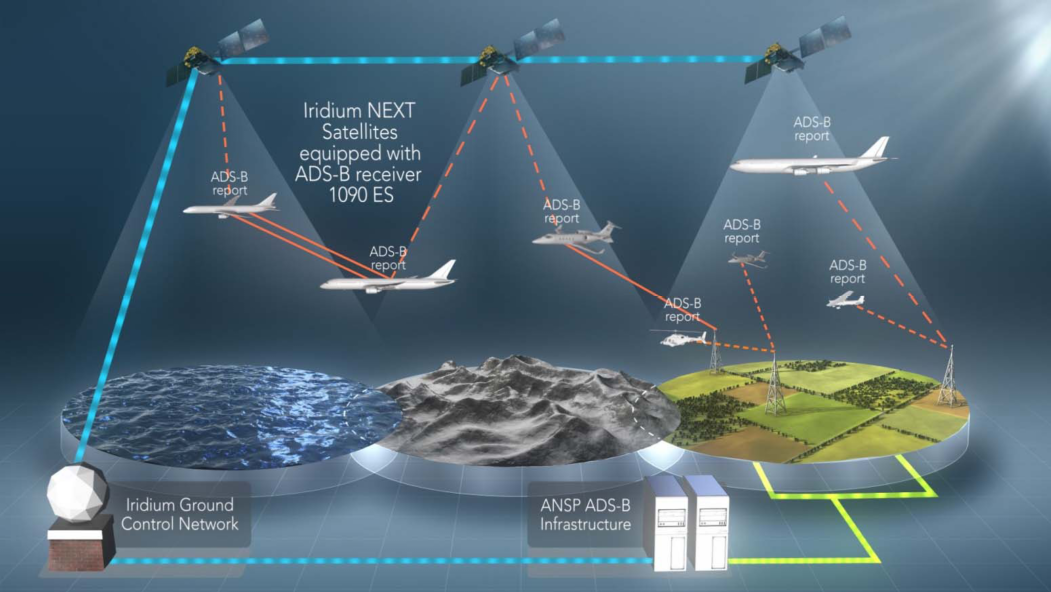
\includegraphics[scale = 0.55]{Pictures/aireon_concept.png}
	
	\caption[Aireon System Concept]{Aireon System Concept, reproduced from \cite{Dawson2013}}
	\label{fig:aireon_concept}
	\end{figure}

Details on the intended orbit and performance standards for the Iridium NEXT constellation had not yet been made publicly available. Descriptions of the Iridium NEXT's intended services suggested that the orbital configuration and control model would be similar to the first Iridium constellation discussed in Section \ref{sec:iridium}  \cite{ADS-B:Aireon_brochure}. 

Although this provided the complete coverage required by the problem statement, it was expected that the cost-model for the system will be quite high. The launch and operations of the first Iridium constellation was complex and costly enough such that mismanagement of the project's investment and return resulted in Iridium filing for bankruptcy a year after the launch of the final satellite in August 1999 \cite{Finkelstein2000}.   The total project and operations cost of a smaller CubeSat constellation would be much lower and therefore have significantly less risk. The solution put forward in this thesis could prove to be more economically effective.

\subsection{Spaced Based ADS-B In-Orbit Demonstration Payload (SABIP)} \label{sec:sadip}
SABIP was presented as space-based ADS-B receiver system designed to operate over the standard Mode S 1090MHz carrier signal currently being developed by Thales Alenia Space Deutschland. The successful implementation of this receiver would enable ADS-B signals to be relayed from LEO without extra infrastructural cost. Specifically, existing Mode S transponders used by aircraft and ANSPs could still be used without significant augmentation to existing equipment. The system was intended to receive and record ADS-B messages, decode those messages and then assemble reports that can be transmitted to ground stations and ANSPs \cite{Blomenhofer2012}. 

The research put forward that the chief challenge in designing the receiver was mitigating signal degradation due to high-density traffic. The Mode S frequency is time-shared for both ADS-B transmissions and Traffic Collision Avoidance Systems (TCAS) for all aircraft. The enlarged antenna footprint from LEO meant that both of these signals need to be detected and processed for a high number of aircraft. The footprint of a receiver from LEO would have a radius of approximately 3200 nautical miles whilst a terrestrial Mode S receivers typically have a footprint of 200 nautical miles. This degraded the detection of squitter signals over Mode S transmission \cite{Blomenhofer2012}. 

The proposed solution consisted of an ADS-B antenna which has multiple spot beams, each covering a limited area. The models of this antenna are shown in Figure \ref{fig:sapid_spotbeams}. The exact number and configuration of spot beams had yet to be determined and required further study of signal degradation due to transmission density \cite{Blomenhofer2012}.

\begin{figure}[htb]
	\centering
	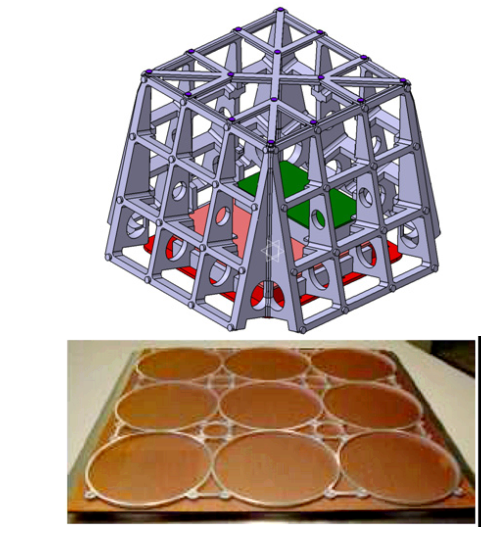
\includegraphics[scale = 0.8]{Pictures/sapid_spotbeams.png}
	
	\caption[SAPID receiver Antenna design]{SABIP receiver Antenna design, reproduced from \cite{Blomenhofer2012}}
	\label{fig:sapid_spotbeams}
\end{figure}

This research identified the key need to deal with signal collisions and maintaining a high probability of aircraft detection. In particular, the issues with detection probability given a high number of aircraft agree with the Mode S receiver requirements described in \cite{Orlando2001}. This means that re-visit time and scan time for a particular area on Earth will be key parameters in evaluating the effectiveness of any given ADS-B constellation

The technology developed by Thales could also form a foundation for the implementation of a CubeSat based ADS-B receiver system. Signal collision and resolution problems outlined in the paper would be experienced by any in-orbit ADS-B receiver. Although the exact antenna dimensions prohibit SABIP from being incorporated into a CubeSat form-factor, the same design principles would need to be incorporated into a the design of a more suitably sized receiver. Similarly the data storage and analysis framework put forward in \cite{Blomenhofer2012} could be used for the ground and space segment of the ADS-B system. The research indicated that the technology required for a spaced based ADS-B receiver is certainly possible in the CubeSat form factor.


\subsection{Proba V}
In early 2013, the European Space Agency (ESA) launched their fifth experimental Proba satellite, Proba V, with a guest ADS-B Payload. Like SABIP, the ADS-B payload is designed to receive signals via the native Mode S 1090Mhz carrier. The receiver, designed by the German Aerospace Center (DLR) was designed to receive ADS-B from LEO in Proba V's 820km orbit \cite{DLR,TheEur,T}. Proba V is travelling in a Sun-Synchronus polar orbit at an altitude of 820km \cite{TheEur}.  

As of June 2014, the satellite was tracking Aircraft over Northern Europe \cite{DLR}. Tests to determine the sensitivity of the receiver to issues caused by signal density (as put forward by \cite{Blomenhofer2012}) were ongoing. Figure \ref{fig:probav_planes} shows the results from the initial proof of concept, with aircraft being detected in Europe\cite{TheEur}. No further results beyond this proof of concept have been published. However this provided further evidence for the viability of receiving ADS-B signals from LEO, particularly from an altitude as high as 820km.
\begin{figure}[H]
	\centering
	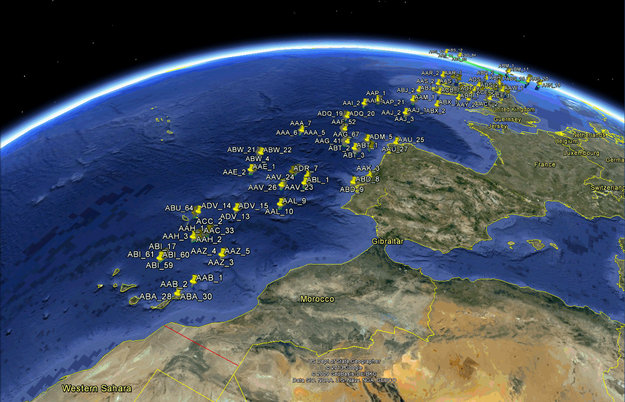
\includegraphics[scale = 0.5]{Pictures/probav_planes.jpg}
	
	\caption[Aircraft detected by Proba V over Europe]{Aircraft detected by Proba V over Europe, reproduced from \cite{TheEur}}
	\label{fig:probav_planes}
\end{figure}

\subsection{GOM-X1} \label{sec:gomx}
The GOM-X1 was a 2U CubeSat intended to perform a number of space based experiments using software defined radio (SDR), the primary being a a spaced based ADS-B receiver. The satellite was developed as a collaborative effort between GomSpace, DSE Airport Solutions (now Insero Software \cite{Insero2014}) and Aalborg University. The primary mission of the satellite was to demonstrate that ADS-B reception is capable from a CubeSat platform in LEO. Data received from onboard sensors would be compared with ground-based ADS-B data to verify the correctness of the data acquired from LEO\cite{GomSpace2014,Alminde2012}.

ADS-B signals were to be received via a custom SDR payload. The SDR is designed to be able to have a reconfigurable decoder structure. The intention of the experiments was to evaluate the effectiveness of different decoder configurations. This data would be used for further refinements to space based ADS-B CubeSat modules. A helical receiver antenna is used in order to maximise the gain going into the system, pictured in Figure \ref{fig:gomx_antenna}.  GOM-X1 used a standard commercially off-the-shelf (COTS) bus available from GomSpace\cite{Alminde2012}.
\begin{figure}[H]
	\centering
	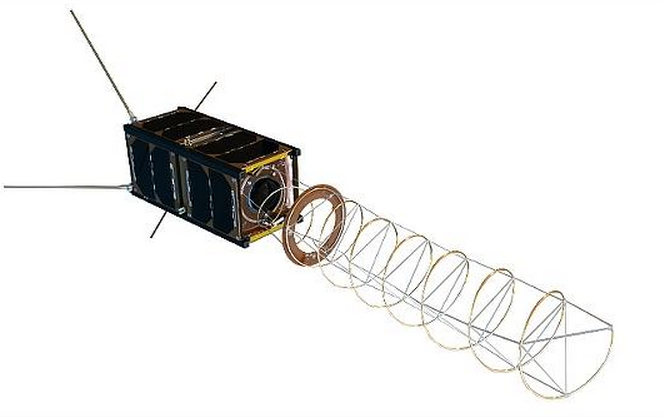
\includegraphics[scale = 0.5]{Pictures/gomx_antenna.png}
	
	\caption[3D render of the GOM-X1 satellite, showing the expanded helical receiver antenna]{3D render of the GOM-X1 satellite, showing the expanded helical receiver antenna, reproduced from \cite{GomSpace2014}}
	\label{fig:gomx_antenna}
\end{figure}
The satellite was successfully launched in November of 2013 into an circular orbit of 600km altitude and 97.8 degrees of inclination. GOM-X was still `fully commissioned' and operational in June of 2014\cite{EoPortal, GomSpace2014}. GomSpace released a `preliminary plot' of the received aircraft positions, reproduced in Figure \ref{fig:gomx_planes}, showing detected aircraft mostly in the northern hemisphere. 

\begin{figure}[htbp]
	\centering
	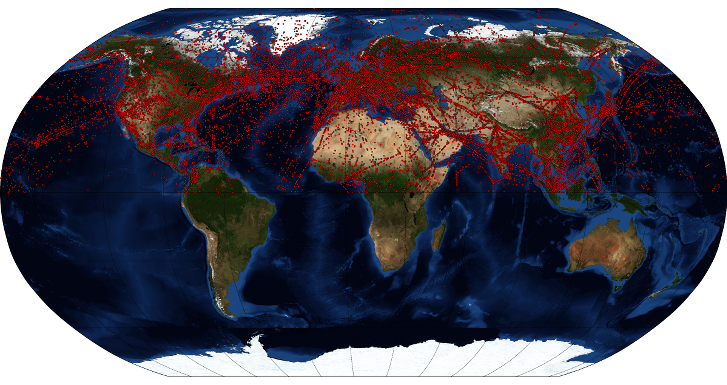
\includegraphics[scale = 0.8]{Pictures/gomx_planes.png}
	
	\caption[Preliminary plot of planes detected by GOM-X1]{Preliminary plot of planes detected by GOM-X1, reproduced from \cite{GomSpace2014}}
	\label{fig:gomx_planes}
\end{figure}

The early success of the mission provides a good indication of the viability of a CubeSat based ADS-B receiver. However no data is provided on the quantitative performance of the receiver. Of particular interest would be the aircraft detection rate of a given pass or scan of the satellite. Being able to determine the statistical likelihood of aircraft detection from the GOM-X1 would provide a hard systems constraint for the design of a CubeSat constellation. The data presented in this thesis will instead provide a range of constraints on the sensitivity of the required ADS-B receiver from the analysis of proposed constellations  


\begin{comment}
\subsection{Automatic Identification System (AIS)}
The Automatic Identification System (AIS) is the maritime analogue to ADS-B. The system consists of VHF transponders which relay ship telemetry (identity, heading, destination etc.) between ships and between ships and shore stations. The viability of augmenting AIS with a LEO space-segment has been in investigation since 2003 \cite{Hoye2008}. The primary goal of the proposed Satellite AIS systems is to provide route monitoring, allowing for longer update periods and data-lag. 

\subsubsection{Satellite-based Receivers}
The key challenge with Satellite-based AIS, as with ADS-B, is the detection of signals in high density areas where signal collision is prominent. Low density areas with less than 2000 ships will yield a detection rate of 99\% from conventional AIS receivers \cite{Hoye2008, Carson-Jackson2012}. This number drops off significantly as more ships enter the antenna footprint, dropping as low as 50\% with 2500 ships for an observation time of 15 minutes \cite{Hoye2008}. There are two design solutions to mitigate this issue \cite{Hoye2008, Carson-Jackson2012, Scorzolini2010}:
\begin{itemize}
	\item Increase observation time by decreasing the period between satellite revisits and allowing multiple passes to happen over a given area. This introduces extra infrastructural costs, requiring more satellites and ground stations to maintain 
	\item Designing AIS receivers to have narrow-footprint spot beams, decreasing the number of ships and chance of signal collision for a particular receiver. This decreases the area of effectiveness for one satellite and may necessitate more satellites to support the entire system.
\end{itemize}
Both exactEarth \cite{Exact} and ORBCOMM \cite{ORBCOMM} produce AIS receivers designed for flight on LEO micro-satellites. ORBCOMM have launched two LEO satellites containing their AIS receiver, one in an equatorial orbit and the other in a polar orbit. The company claims that these two satellites provide "complete global AIS coverage" but do not specify at what update rate. ORBCOMM will launch an additional 17 AIS equipped LEO satellites in 2013 at unspecified orbital configurations \cite{ORBCOMM}. The current ORBCOMM constellation is inclined at various inclinations and altitudes, determined by system requirements at time of individual satellite deployment \cite{Tandler1996}.

\subsubsection{Proposed Constellations}
The constellation designs put forward for Satellite AIS are less ambitious than Space Based ADS-B solutions, providing longer update rates. \cite{Hoye2008} claims that four constellations in 4 identical and equally spaced orbital planes at an inclination of $58^\circ$ will provide  global coverage with an update rate of once per hour. This figure can be doubled with 8 satellites \cite{Hoye2008}.

A study released by the Telespazio puts forward three scenarios, each dependant on the nature of the ground-station network\cite{Scorzolini2010}:
\begin{enumerate}
	\item Six satellites in six sun synchronous orbits delivering an update rate of less than 3 hours. The revisit time for each point on Earth would be less than 2 hours. The data would have an update lag of 1 hour.
	\item Twelve satellites in 6 orbital planes with an update rate of less than one hour. This number would increase to 25 if multiple passes are needed to ensure detection integrity. The update lag is claimed to be lower than 30 minutes.
	\item Ten satellites in an unspecified orbit with an update time of 1.5 hours and update lag of 45 minutes.
\end{enumerate}
The exact orbital configuration and ground station network was not specified.

An ESA sutdy specifies an AIS system with a 3 hour reporting interval that uses  6-8 Satellites at an altitude of approximately 600km "with proper orbit design" \cite{Cervera2008}. This study is expanded upon in \cite{Cervera2011}, where 5 LEO satellites are suggested to be in 5 different orbital planes each with $30^\circ$ difference in RAAN. Inclinations of between $80^\circ$ and $100^\circ$ were suggested, each having different coverage and revisit time trade-offs. Up to 10 satellites in the same configuration may be necessary for high population ship cases \cite{Cervera2011}. 

The performance parameters for each of the Satellite AIS systems investigated do not meet the immediacy requirements of ADS-B. The proposed AIS constellation designs can be mimicked in order to provide basic route monitoring for aircraft, but not live tracking data. However, the technologies investigated and basic system design provide a good base model from which a more immediate system can be designed. In particular, having more satellites and implementing inter-satellite links as per Iridium can drastically improve the update time performance of the proposed system. 

\end{comment}

\subsection{Conclusions}
The survey of current technologies show that there is commercial motivation for the development of ADS-B systems from Space.  ALAS and Aireon represent significant commercial investment in the development of space based ADS-B systems. Although the large commercial risk is absorbed significantly by having the payloads `piggy-back' on the Globalstar and Iridium NEXT constellations, the costs of the buy-in model are not yet known. 

Proba V, SABIP and GOM-X1 demonstrate that there is significant interest in implementing space-based ADS-B on small satellites. Proba V and SABIP are both designed for use on smaller  satellites with the intention of potentially lowering the cost of a space based ADS-B system. Proba V in particular has already demonstrated success, though the quantification of that success is not yet known. The success of GOM-X1 proves that the technology is viable on a CubeSat scale.

These examples show that there is ongoing interest and motivation in developing an economic solution for a space based ADS-B system. The Iridium NEXT and Globalstar constellations provide guaranteed system update and coverage but the design is not necessarily optimised for ADS-B coverage. Given the success of technology demonstrators for small satellites, there is sufficient motivation for development of a low cost ADS-B constellation using CubeSats. 